%% bt: Bachelor Thesis
%% mt: Master Thesis
\documentclass[ngerman,bt]{dbvdoc}

% Alternative Loesunge:
% - use utf8 on your home computer
% - use an editor capable of converting character-sets and editing utf8 files
%   on a latin1 system (some versions of vi do)
% - use \"{a}, \"{o}, \"{u}, \ss{} instead of non-ascii characters

\usepackage[utf8]{inputenc}
%%\usepackage[utf8,latin1]{inputenc}  %% Alternative Eingabe
\usepackage{babel}
\usepackage[babel,german=quotes]{csquotes}
\usepackage[backend=biber,maxnames=99,language=german,bibstyle=alphabetic,sortcites=true,labelalpha=true]{biblatex}
\usepackage{hyperref}
\usepackage{breakurl}
%\usepackage[hyphenbreaks]{breakurl}  %% Falls in \url auch bei Bindestrich getrennt werden soll. Weitere Optionen: RTFM
\usepackage{graphicx}
\usepackage{epsfig}
\usepackage{subfigure}
\usepackage{psfrag}
\usepackage{color}

% \setcounter{lotdepth}{2}

% ++ es werden keine underfull hboxes als Fehler ausgegeben,
%    da das ja nur heißt, dass die Seite noch nicht ganz voll ist
\hbadness=10000
\clubpenalty = 10000 % schliesst Schusterjungen aus
\widowpenalty = 10000 % schliesst Hurenkinder aus

\pagenumbering{roman}

%\bibliographystyle{galpha2a}
\renewcommand*{\labelalphaothers}{\textsuperscript{}} %% plus-zeichen abschalten
\bibliography{doc}
\addbibresource{doc.bib}
\addbibresource{lit.bib}

%%%%%%%%%%%%%%
%%% MACROS %%%
%%%%%%%%%%%%%%
%% if macros shall be used, put them into a separate file 'macros.tex'
%%\input{macros}

%%%%%%%%%%%%%%%%%%%%
%%% Worttrennung %%%
%%%%%%%%%%%%%%%%%%%%
%% if hyphenation patterns are needed, put them into a separate file 'hyph.tex'
%%\input{hyph}


%%%%%%%%%%%%%%
%\setcounter{tocdepth}{5}
%\setcounter{secnumdepth}{5}

\sloppy		%% avoid writing over linebreak


\begin{document}
\clearpage
  \selectlanguage{\ngerman}
  \begin{deckblatt}
    \Titel{Simulating Room Acoustics Using Ray Tracing}
    \Name{Reichel}
    \Vorname{Christina}
    \Wohnort{Würzburg}
    \BetreuerA{Erstpr\"{u}fer: Prof.~Dr.-Ing.~Frank Deinzer}
    \BetreuerB{Zweitpr\"{u}fer: Prof.~Dr.-Ing.~Arndt Balzer}
    \Ende{2. 04. 2024}
    \Fach{Informatik}
    \Schwerpunkt{Medieninformatik}
    \Angefertigt{Angefertigt an der Fakultät für Informatik und Wirtschaftsinformatik der Technischen Hochschule Würzburg-Schweinfurt}
  \end{deckblatt}
\clearpage
\mbox{}
\vfill
\begin{center}
\ifpdf
	
\includegraphics[width=6cm]{qrcode-thesis.png}
\else
	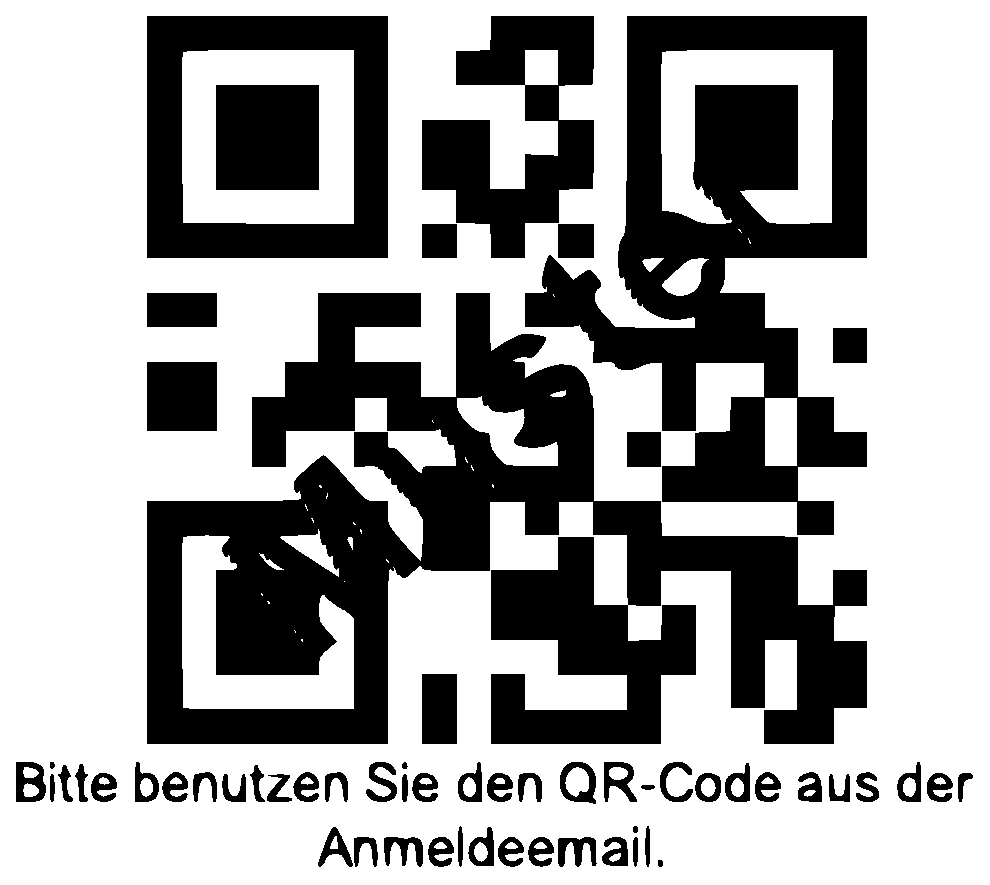
\includegraphics[width=6cm]{qrcode-thesis.eps}
\fi
\end{center}
\clearpage

\noindent Hiermit versichere ich, dass ich die vorgelegte Bachelorarbeit/Masterarbeit selbstständig verfasst und noch nicht
anderweitig zu Prüfungszwecken vorgelegt habe. Alle benutzten Quellen und Hilfsmittel sind
angegeben, wörtliche und sinngemäße Zitate wurden als solche gekennzeichnet.\\[5mm]
Würzburg, den\\[20mm]
(Unterschrift)

\vfill

\noindent Hiermit willige ich ein, dass zum Zwecke der Überprüfung auf Plagiate meine vorgelegte Arbeit in
digitaler Form an PlagScan übermittelt und diese vorübergehend (max. 5 Jahre)
in der von PlagScan geführten Datenbank gespeichert wird, sowie persönliche Daten, die Teil dieser
Arbeit sind, dort hinterlegt werden.

Die Einwilligung ist freiwillig. Ohne diese Einwilligung kann unter Entfernung aller persönlichen
Angaben und Wahrung der urheberrechtlichen Vorgaben die Plagiatsüberprüfung nicht verhindert
werden. Die Einwilligung zur Speicherung und Verwendung der persönlichen Daten kann jederzeit
durch Erklärung gegenüber der Fakultät widerrufen werden.\\[5mm]
Würzburg, den\\[20mm]
(ggf. Unterschrift)

\clearpage

\begin{center}
\bf Übersicht
\end{center}
TEXT DEUTSCH


\vfill
\begin{center}
\bf Abstract
\end{center}
TEXT ENGLISCH

\vfill
\cleardoublepage

\tableofcontents

\cleardoublepage \pagenumbering{arabic}

%%%%%%%%%%%%%%%%%%%%%%%
%%% Inlucde chapter %%%
%%%%%%%%%%%%%%%%%%%%%%%
\chapter{Einleitung}

Zitat: \cite{Bronstein08:TDM,LongURL}.

Lorem ipsum dolor sit amet, consectetuer adipiscing elit. Aenean commodo ligula 
eget dolor. Aenean massa. Cum sociis natoque penatibus et magnis dis parturient 
montes, nascetur ridiculus mus. Donec quam felis, ultricies nec, pellentesque 
eu, pretium quis, sem. Nulla consequat massa quis enim. Donec pede justo, 
fringilla vel, aliquet nec, vulputate eget, arcu. In enim justo, rhoncus ut, 
imperdiet a, venenatis vitae, justo. Nullam dictum felis eu pede mollis pretium. 
Integer tincidunt. Cras dapibus. Vivamus elementum semper nisi. Aenean vulputate 
eleifend tellus. Aenean leo ligula, porttitor eu, consequat vitae, eleifend ac, 
enim. Aliquam lorem ante, dapibus in, viverra quis, feugiat a, tellus. Phasellus 
viverra nulla ut metus varius laoreet. Quisque rutrum. Aenean imperdiet. Etiam 
ultricies nisi vel augue. Curabitur ullamcorper ultricies nisi. Nam eget dui. 
Etiam rhoncus. Maecenas tempus, tellus eget condimentum rhoncus, sem quam semper 
libero, sit amet adipiscing sem neque sed ipsum. Nam quam nunc, blandit vel, 
luctus pulvinar, hendrerit id, lorem. Maecenas nec odio et ante tincidunt 
tempus. Donec vitae sapien ut libero venenatis faucibus. Nullam quis ante. Etiam 
sit amet orci eget eros faucibus tincidunt. Duis leo. Sed fringilla mauris sit 
amet nibh. Donec sodales sagittis magna. Sed consequat, leo eget bibendum 
sodales, augue velit cursus nunc, 

\begin{equation}
\vec{v} = \vec{f(\mat{A})} = |{\cal C}| \cdot \argmax_{\mat{A}}  \sum_i{\mat{A}\vec{A}_i}
\quad\forall\mat{A}\in{\cal C}
\end{equation}

Check math\footnote{In einer technischen Arbeit braucht man sehr sehr wenige Fußnoten; meistens gar keine in der ganzen Arbeit}:
%
\begin{equation}
a, A, \vec{a}, \mat{A}, \alpha, \Sigma, \vec{\alpha}, \mat{\Sigma}
\end{equation}

Sed ut perspiciatis unde omnis iste natus error sit voluptatem accusantium 
doloremque laudantium, totam rem aperiam, eaque ipsa quae ab illo inventore 
veritatis et quasi architecto beatae vitae dicta sunt explicabo. Nemo enim ipsam 
voluptatem quia voluptas sit aspernatur aut odit aut fugit, sed quia 
consequuntur magni dolores eos qui ratione voluptatem sequi nesciunt. Neque 
porro quisquam est, qui dolorem ipsum quia dolor sit amet, consectetur, adipisci 
velit, sed quia non numquam eius modi tempora incidunt ut labore et dolore 
magnam aliquam quaerat voluptatem. Ut enim ad minima veniam, quis nostrum 
exercitationem ullam corporis suscipit laboriosam, nisi ut aliquid ex ea commodi 
consequatur? Quis autem vel eum iure reprehenderit qui in ea voluptate velit 
esse quam nihil molestiae consequatur, vel illum qui dolorem eum fugiat quo 
voluptas nulla pariatur? At vero eos et accusamus et iusto odio dignissimos 
ducimus qui blanditiis praesentium voluptatum deleniti atque corrupti quos 
dolores et quas molestias excepturi sint occaecati cupiditate non provident, 
similique sunt in culpa qui officia deserunt mollitia animi, id est laborum et 
dolorum fuga. Et harum quidem rerum facilis est et expedita distinctio. Nam 
libero tempore, cum soluta nobis est eligendi optio cumque nihil impedit quo 
minus id quod maxime placeat facere 

Li Europan lingues es membres del sam familie. Lor separat existentie es un 
myth. Por scientie, musica, sport etc, litot Europa usa li sam vocabular. Li 
lingues differe solmen in li grammatica, li pronunciation e li plu commun 
vocabules. Omnicos directe al desirabilite de un nov lingua franca: On refusa 
continuar payar custosi traductores. At solmen va esser necessi far uniform 
grammatica, pronunciation e plu sommun paroles. Ma quande lingues coalesce, li 
grammatica del resultant lingue es plu simplic e regulari quam ti del coalescent 
lingues. Li nov lingua franca va esser plu simplic e regulari quam li existent 
Europan lingues. It va esser tam simplic quam Occidental in fact, it va esser 
Occidental. A un Angleso it va semblar un simplificat Angles, quam un skeptic 
Cambridge amico dit me que Occidental es. Li Europan lingues es membres del sam 
familie. Lor separat existentie es un myth. Por scientie, musica, sport etc, 
litot Europa usa li sam vocabular. Li lingues differe solmen in li grammatica, 
li pronunciation e li plu commun vocabules. Omnicos directe al desirabilite de 
un nov lingua franca: On refusa continuar payar custosi traductores. At solmen 
va esser necessi far uniform grammatica, pronunciation e plu sommun paroles. 

Lorem ipsum dolor sit amet, consectetuer adipiscing elit. Aenean commodo ligula 
eget dolor. Aenean massa. Cum sociis natoque penatibus et magnis dis parturient 
montes, nascetur ridiculus mus. Donec quam felis, ultricies nec, pellentesque 
eu, pretium quis, sem. Nulla consequat massa quis enim. Donec pede justo, 
fringilla vel, aliquet nec, vulputate eget, arcu. In enim justo, rhoncus ut, 
imperdiet a, venenatis vitae, justo. Nullam dictum felis eu pede mollis pretium. 
Integer tincidunt. Cras dapibus. Vivamus elementum semper nisi. Aenean vulputate 
eleifend tellus. Aenean leo ligula, porttitor eu, consequat vitae, eleifend ac, 
enim. Aliquam lorem ante, dapibus in, viverra quis, feugiat a, tellus. Phasellus 
viverra nulla ut metus varius laoreet. Quisque rutrum. Aenean imperdiet. Etiam 
ultricies nisi vel augue. Curabitur ullamcorper ultricies nisi. Nam eget dui. 
Etiam rhoncus. Maecenas tempus, tellus eget condimentum rhoncus, sem quam semper 
libero, sit amet adipiscing sem neque sed ipsum. Nam quam nunc, blandit vel, 
luctus pulvinar, hendrerit id, lorem. Maecenas nec odio et ante tincidunt 
tempus. Donec vitae sapien ut libero venenatis faucibus. Nullam quis ante. Etiam 
sit amet orci eget eros faucibus tincidunt. Duis leo. Sed fringilla mauris sit 
amet nibh. Donec sodales sagittis magna. Sed consequat, leo eget bibendum 
sodales, augue velit cursus nunc, 

Sed ut perspiciatis unde omnis iste natus error sit voluptatem accusantium 
doloremque laudantium, totam rem aperiam, eaque ipsa quae ab illo inventore 
veritatis et quasi architecto beatae vitae dicta sunt explicabo. Nemo enim ipsam 
voluptatem quia voluptas sit aspernatur aut odit aut fugit, sed quia 
consequuntur magni dolores eos qui ratione voluptatem sequi nesciunt. Neque 
porro quisquam est, qui dolorem ipsum quia dolor sit amet, consectetur, adipisci 
velit, sed quia non numquam eius modi tempora incidunt ut labore et dolore 
magnam aliquam quaerat voluptatem. Ut enim ad minima veniam, quis nostrum 
exercitationem ullam corporis suscipit laboriosam, nisi ut aliquid ex ea commodi 
consequatur? Quis autem vel eum iure reprehenderit qui in ea voluptate velit 
esse quam nihil molestiae consequatur, vel illum qui dolorem eum fugiat quo 
voluptas nulla pariatur? At vero eos et accusamus et iusto odio dignissimos 
ducimus qui blanditiis praesentium voluptatum deleniti atque corrupti quos 
dolores et quas molestias excepturi sint occaecati cupiditate non provident, 
similique sunt in culpa qui officia deserunt mollitia animi, id est laborum et 
dolorum fuga. Et harum quidem rerum facilis est et expedita distinctio. Nam 
libero tempore, cum soluta nobis est eligendi optio cumque nihil impedit quo 
minus id quod maxime placeat facere 

Li Europan lingues es membres del sam familie. Lor separat existentie es un 
myth. Por scientie, musica, sport etc, litot Europa usa li sam vocabular. Li 
lingues differe solmen in li grammatica, li pronunciation e li plu commun 
vocabules. Omnicos directe al desirabilite de un nov lingua franca: On refusa 
continuar payar custosi traductores. At solmen va esser necessi far uniform 
grammatica, pronunciation e plu sommun paroles. Ma quande lingues coalesce, li 
grammatica del resultant lingue es plu simplic e regulari quam ti del coalescent 
lingues. Li nov lingua franca va esser plu simplic e regulari quam li existent 
Europan lingues. It va esser tam simplic quam Occidental in fact, it va esser 
Occidental. A un Angleso it va semblar un simplificat Angles, quam un skeptic 
Cambridge amico dit me que Occidental es. Li Europan lingues es membres del sam 
familie. Lor separat existentie es un myth. Por scientie, musica, sport etc, 
litot Europa usa li sam vocabular. Li lingues differe solmen in li grammatica, 
li pronunciation e li plu commun vocabules. Omnicos directe al desirabilite de 
un nov lingua franca: On refusa continuar payar custosi traductores. At solmen 
va esser necessi far uniform grammatica, pronunciation e plu sommun paroles. 

    
\cleardoublepage
%\include{doc02}   
%\cleardoublepage
%% usw.
\nocite{*}  %% Das ist nur zu Demo-Zwecken da!
%%%%%%%%%%%%%%
%%% Anhang %%%
%%%%%%%%%%%%%%
%\begin{appendix}
%\include{doc-a0} 
%\cleardoublepage
%\include{doc-a1} 
%\cleardoublepage
%%usw...
%\end{appendix}

%% Literatur
\addcontentsline{toc}{chapter}{\bibname}
\printbibliography
\cleardoublepage

%% Bilderverzeichnis
\addcontentsline{toc}{chapter}{\listfigurename}
\listoffigures\cleardoublepage

%% Tabellenverzeichnis
\addcontentsline{toc}{chapter}{\listtablename}
\listoftables\cleardoublepage


\end{document}
